\documentclass[10pt,a4paper,twocolumn]{article}
\usepackage[utf8]{inputenc}
\usepackage[T1]{fontenc}
\usepackage[spanish]{babel}
\usepackage{amsmath}
\usepackage{amsfonts}
\usepackage{amssymb}
\usepackage{graphicx}
\usepackage{geometry}
\usepackage{xcolor}
\usepackage{fancyhdr}
\usepackage{microtype}
\usepackage{caption}
\usepackage{titlesec}
\usepackage{enumitem}
\usepackage{booktabs}
\usepackage{tabularx}
\usepackage{needspace}
\usepackage{hyperref}

\geometry{
    top=3.0cm, bottom=1.8cm, left=1.8cm, right=1.8cm,
    headheight=42pt, headsep=12pt
}
\hypersetup{
    colorlinks=true,
    linkcolor=blue!50!black,
    citecolor=blue!50!black,
    urlcolor=blue!50!black,
    pdftitle={Hacia la resolución de la materia exótica en la métrica de Alcubierre},
    pdfsubject={Propagación de estado y límites causales en la TCDS}
}
\captionsetup{font=small,labelfont=bf}
\setlength{\emergencystretch}{2em}
\setlength{\columnsep}{0.7cm}
\setlength{\parindent}{1em}
\setlength{\textfloatsep}{12pt plus 2pt minus 2pt}
\setlength{\intextsep}{10pt plus 2pt minus 2pt}
\setlist[itemize]{leftmargin=*,itemsep=2pt,topsep=4pt,parsep=0pt}
\titleformat{\section}{\normalfont\large\bfseries}{\thesection.}{0.5em}{}
\titleformat{\subsection}{\normalfont\normalsize\bfseries}{\thesubsection.}{0.5em}{}
\titlespacing*{\section}{0pt}{10pt plus 2pt minus 2pt}{5pt}
\titlespacing*{\subsection}{0pt}{8pt plus 2pt minus 2pt}{4pt}
\raggedbottom

\newcounter{parrafoecuacion}
\newcommand{\parrafoecuacion}[2]{%
    \par\smallskip\Needspace{6\baselineskip}%
    \noindent\refstepcounter{parrafoecuacion}\label{#1}%
    \textbf{P\theparrafoecuacion.\ #2.}\enspace
}
\newcommand{\entradaecuacion}[4]{%
    \item[\eqref{#1}\ #3] #4
    Véase el párrafo~\hyperref[#2]{P\ref*{#2}},
    p.~\pageref{#2}.
}

\newcommand{\encabezadoTCDS}{%
    \fancyhf{}%
    \fancyhead[L]{\includegraphics[height=1.3cm]{prism-uploads/images_logo_tcds.png}}%
    \fancyhead[R]{\small\textsc{TCDS}\quad Documento de trabajo}%
    \fancyfoot[C]{\thepage}%
    \renewcommand{\headrulewidth}{0.4pt}%
    \renewcommand{\footrulewidth}{0pt}%
}
\pagestyle{fancy}
\encabezadoTCDS
\fancypagestyle{plain}{\encabezadoTCDS}

\title{\textbf{Hacia la resolución de la materia exótica en la métrica de Alcubierre}\\[0.5em]
    \large Propagación de estado y límites causales en la Teoría Cromodinámica Sincrónica (TCDS)}
\author{Documento de trabajo / Propuesta teórica\\[0.4em]
    \small ORCID: \href{https://orcid.org/0009-0005-6358-9910}{0009-0005-6358-9910}}
\date{\today}

\begin{document}

\twocolumn[
\begin{@twocolumnfalse}
\maketitle

\begin{abstract}
Este documento presenta una reestructuración topológica de la métrica de Alcubierre~\cite{alcubierre1994}. Mediante la Teoría Cromodinámica Sincrónica (TCDS), se demuestra que la deformación del espacio-tiempo no requiere densidades de energía negativa infinita, sino que opera como una propagación de estado sobre una red discreta, acotada por una fricción topológica finita ($\varphi$) y una tasa máxima de actualización causal ($K_{\text{RATE}}$).
\end{abstract}
\vspace{1em}
\end{@twocolumnfalse}
]

\paragraph{Antecedente y alcance de la referencia.}
El Dr. M. Alcubierre~\cite{alcubierre1994} propuso una geometría relativista con expansión del espacio detrás de una nave y contracción delante de ella, que permite un movimiento global superlumínico y requiere materia exótica. Se cita ese trabajo como antecedente geométrico, no como una validación de la TCDS. La red discreta, sus constantes y las conclusiones que siguen corresponden a la propuesta de este documento.
Como referencia general sobre relatividad numérica se incluye el libro \textit{Introduction to 3+1 Numerical Relativity}, de Alcubierre~\cite{alcubierre2008}. Se incorpora asimismo la referencia adicional de Zenodo~\cite{zenodo22639220}.

\section{Interpretación de la divergencia y límite de continuidad}
\label{sec:interpretacion-divergencia}

Al derivar la métrica de deformación, se encuentra que el tensor de energía-momento requiere densidades negativas que divergen en ciertas regiones. En el marco de espacio continuo donde originalmente se formuló esta solución, dicha divergencia se ha interpretado durante décadas como la necesidad de cantidades arbitrariamente grandes de energía exótica, lo que ha llevado a considerar la métrica físicamente irrealizable. Sin embargo, es fundamental distinguir entre una propiedad intrínseca de la curvatura y un artefacto del modelo matemático empleado. La divergencia no surge de la geometría en sí misma, sino de integrar sobre un dominio infinitamente divisible. Si se admite que el sustrato físico posee una granularidad mínima indivisible \(L_{\text{min}}\), la integral se trunca naturalmente y el resultado deja de ser infinito, transformándose en un valor finito y constante: una fricción topológica del propio sustrato, denotada \(\phi\).

Bajo esta perspectiva, el perfil de deformación no requiere que la nave se desplace a través del espacio. En su lugar, el estado de compresión frontal y relajación trasera se transmite secuencialmente de un nodo al siguiente del sustrato, como una onda de estado sin traslación material. La velocidad de propagación de la burbuja queda limitada estrictamente por la frecuencia máxima de actualización de la red \(K_{\text{RATE}} = c / L_{\text{min}}\), nunca superando \(c\) y respetando estrictamente la causalidad. Se concluye que el requerimiento de energía exótica infinita no era una propiedad del mecanismo warp, sino el costo de asumir continuidad donde existe granularidad.
% ==============================================================================
% MARCO ALGEBRAICO TCDS — DESDE PRIMEROS PRINCIPIOS (LBCU)
% Forma puramente adimensional · Sin parámetros libres · Sin energía exótica
% ==============================================================================

\section{Marco algebraico desde primeros principios}
\label{sec:marco_lbcu}

\Needspace{10\baselineskip}
\subsection{Postulado fundamental: Ley de Balance Coherencial Universal (LBCU)}
\parrafoecuacion{par:lbcu}{Balance coherencial}
Toda deformación del sustrato se rige por una relación de equilibrio entre tres magnitudes adimensionales, sin constantes externas ni parámetros libres:
\begin{equation}
    Q \cdot \Sigma \cdot \tau_C = \phi.
    \label{eq:lbcu}
\end{equation}
Las magnitudes de la ecuación~\eqref{eq:lbcu} se definen como sigue:
\begin{description}[style=nextline,leftmargin=1em,labelindent=0pt,itemsep=4pt,parsep=0pt]
    \item[$Q$: coherencia del perfil.]
    Grado de coherencia o integridad del perfil, con $0 < Q \leq 1$; el límite $Q \to 1$ representa la máxima definición.
    \item[$\Sigma$: tensión topológica.]
    Gradiente de tensión topológica del sustrato, con $0 < \Sigma \leq 1$; se considera proporcional al laplaciano del perfil de acoplamiento.
    \item[$\tau_C$: tiempo causal.]
    Tiempo causal de sincronización entre nodos adyacentes, con $-1 \leq \tau_C \leq 1$; su signo indica la dirección de propagación.
    \item[$\phi$: fricción topológica.]
    Fricción finita del sustrato, especificada en la ecuación~\eqref{eq:phi}.
\end{description}

\parrafoecuacion{par:phi}{Fricción del sustrato}
El valor constante de fricción topológica que se presenta en este marco es:
\begin{equation}
    \phi = \frac{1+\sqrt{5}}{2} \approx 1.618034.
    \label{eq:phi}
\end{equation}
No se introduce energía, masa ni densidad exótica. Todos los términos de la LBCU son adimensionales y se definen exclusivamente entre sí.

\Needspace{10\baselineskip}
\subsection{Relaciones que emergen algebraicamente}
De la LBCU se despejan todas las magnitudes sin introducir nada externo.

\parrafoecuacion{par:tiempo-causal}{Tiempo causal}
La relación para el tiempo causal de sincronización se escribe como:
\begin{equation}
    \tau_C = \frac{\phi}{Q \cdot \Sigma}.
    \label{eq:tiempo-causal}
\end{equation}

\parrafoecuacion{par:amplitud}{Amplitud base del desnivel}
La amplitud pura adimensional del desnivel topológico (previo a su proyección en unidades físicas) se expresa mediante:
\begin{equation}
    \kappa_{\text{base}} = -Q \cdot \phi.
    \label{eq:amplitud}
\end{equation}

\parrafoecuacion{par:exponente}{Exponente de la red}
El exponente topológico de la red tridimensional se expresa mediante:
\begin{equation}
    n = 9 \cdot Q \cdot \phi.
    \label{eq:exponente}
\end{equation}
Ninguna de estas cantidades se ajusta a datos experimentales ni se postula por separado: todas emergen de la estructura de la ecuación fundamental.

\Needspace{10\baselineskip}
\subsection{Perfil de acoplamiento y geodésica}
\parrafoecuacion{par:perfil}{Perfil de acoplamiento}
El estado local del sustrato se describe mediante el nivel de acoplamiento $LI(x) \in [0,1]$:
\begin{equation}
    LI(x) = LI_0 + (1-LI_0) \cdot f(x).
    \label{eq:perfil}
\end{equation}
Aquí, $LI_0$ es el estado base del sustrato relajado, también derivado de la condición de frontera $\tau_C \to 1$ cuando $Q \to 0$.

\parrafoecuacion{par:forma}{Función de forma}
La función que interviene en la ecuación~\eqref{eq:perfil} es:
\begin{equation}
    \begin{aligned}
        f(x) = \frac{1}{2}\bigl[&\tanh\!\bigl(10(x+R)\bigr)\\
                              &-\tanh\!\bigl(10(x-R)\bigr)\bigr].
    \end{aligned}
    \label{eq:forma}
\end{equation}

\parrafoecuacion{par:geodesica}{Geodésica de tensión}
La expresión del modelo combina la amplitud base, el exponente y la variación espacial del perfil:
\begin{equation}
    g(x) = -\kappa_{\text{base}} \cdot n \cdot LI(x)^{\,n-1}
           \cdot \left|\frac{dLI}{dx}\right|.
    \label{eq:geodesica}
\end{equation}

\Needspace{10\baselineskip}
\subsection{Costo de fricción topológica: sustituto de la energía exótica}
\parrafoecuacion{par:costo}{Costo local del perfil}
El único costo asociado al mantenimiento del perfil asimétrico es:
\begin{equation}
    T(x) = \left|\frac{dg}{dx}\right| \propto \phi.
    \label{eq:costo}
\end{equation}
$T(x)$ es finito, localizable y acotado. No diverge porque el dominio $x$ no es continuo ni infinitamente divisible: está cuantizado en pasos $\Delta x \geq L_{\text{min}}$. La integral sobre un dominio discreto trunca naturalmente cualquier divergencia potencial.

\Needspace{10\baselineskip}
\subsection{Límite de propagación y causalidad}
\parrafoecuacion{par:limite-causal}{Frecuencia y velocidad límite}
La velocidad máxima de transferencia de estado entre nodos del sustrato viene dada por la frecuencia máxima de sincronización:
\begin{equation}
    \begin{aligned}
        K_{\text{RATE}} &= \frac{c}{L_{\text{min}}},\\
        v_{\text{max}} &= c.
    \end{aligned}
    \label{eq:limite-causal}
\end{equation}
Ningún perfil puede propagarse más rápido que la frecuencia propia del sustrato. La causalidad se respeta estrictamente sin restricciones adicionales.

\Needspace{10\baselineskip}
\subsection{Resumen del sistema cerrado}
Todas las magnitudes se determinan mutuamente. El cuadro siguiente remite a las ecuaciones numeradas; el glosario de la sección~\ref{sec:glosario-ecuaciones} enlaza cada una con su párrafo explicativo.
\begin{center}
    \small
    \setlength{\tabcolsep}{3pt}
    \begin{tabularx}{\linewidth}{@{}>{\raggedright\arraybackslash}X >{\raggedright\arraybackslash}X@{}}
        \toprule
        Magnitud y ecuación & Propiedad\\
        \midrule
        Fricción universal~\eqref{eq:phi} & Constante emergente\\
        Amplitud base~\eqref{eq:amplitud} & Adimensional; sin parámetro libre\\
        Exponente~\eqref{eq:exponente} & Sin parámetro libre\\
        Tiempo causal~\eqref{eq:tiempo-causal} & Despejado de LBCU\\
        Geodésica~\eqref{eq:geodesica} & Derivada del perfil con amplitud base\\
        Costo~\eqref{eq:costo} & Finito, topológico\\
        Límite de velocidad~\eqref{eq:limite-causal} & Imposible superar\\
        \bottomrule
    \end{tabularx}
\end{center}

\Needspace{10\baselineskip}
\subsection{Conclusión del marco}
El sistema es cerrado: todo se deriva de la única ecuación fundamental~\eqref{eq:lbcu}. No existen parámetros libres que requieran ajuste, calibración o medición externa. No se postula energía exótica, materia negativa ni cantidades infinitas. La única aparente divergencia que ha aparecido en modelos anteriores es consecuencia de integrar sobre un espacio continuo idealizado; al reconocer la granularidad del sustrato físico, dicha divergencia se trunca y se convierte en el valor finito y constante de fricción topológica $\phi$.

\section{Postulado I: Límite Causal de la Red Discreta}
El modelo TCDS abandona el continuo espacial en favor de un sustrato granular, estableciendo límites físicos estrictos para la propagación de cualquier deformación topológica:
\parrafoecuacion{par:longitud-minima}{Longitud mínima indivisible}
La escala espacial mínima adoptada para el sustrato es:
\begin{equation}
    L_{\text{min}} = 1.00 \times 10^{-15}\,\mathrm{m}.
    \label{eq:longitud-minima}
\end{equation}

\parrafoecuacion{par:velocidad-maxima}{Velocidad de propagación máxima}
El valor empleado para la velocidad límite es:
\begin{equation}
    c = 3.00 \times 10^8\,\mathrm{m/s}.
    \label{eq:velocidad-maxima}
\end{equation}

\parrafoecuacion{par:frecuencia-maxima}{Frecuencia de actualización máxima}
Con las escalas anteriores, la frecuencia de actualización queda expresada como:
\begin{equation}
    \begin{aligned}
        K_{\text{RATE}} &= \frac{c}{L_{\text{min}}}\\
                       &= 3.00 \times 10^{23}\,\mathrm{Hz}.
    \end{aligned}
    \label{eq:frecuencia-maxima}
\end{equation}
La burbuja de deformación no puede propagarse más rápido de lo que la red se actualiza. $K_{\text{RATE}}$ acota estrictamente la velocidad efectiva a $v \leq c$, eliminando la superluminalidad geométrica y garantizando la preservación de la causalidad sin paradojas temporales.

\section{Postulados II--IV: Propagación de Estado y Costo Energético Finito}
En la TCDS, la nave en el interior de la burbuja warp no experimenta traslación cinética, sino una actualización secuencial del estado de acoplamiento del sustrato circundante.
\parrafoecuacion{par:velocidad-terminal}{Velocidad terminal de la burbuja}
La velocidad terminal propuesta se expresa como:
\begin{equation}
    v = 3.00 \times 10^8\,\mathrm{m/s} = 1.000\,c.
    \label{eq:velocidad-terminal}
\end{equation}

\parrafoecuacion{par:aceleracion-maxima}{Aceleración máxima instantánea}
La aceleración máxima indicada para la actualización del estado es:
\begin{equation}
    \begin{aligned}
        a_{\text{max}} &= c \cdot K_{\text{RATE}}\\
                      &= 8.99 \times 10^{31}\,\mathrm{m/s^2}.
    \end{aligned}
    \label{eq:aceleracion-maxima}
\end{equation}
Dado que no existe desplazamiento de masa en el marco local de la nave, la inercia y las fuerzas G son nulas. El requerimiento de ``materia exótica'' de la geometría de Alcubierre~\cite{alcubierre1994} se sustituye, en esta propuesta, por el peaje de fricción topológica de la red discreta, el cual es estrictamente finito: $\varphi \approx 1.618034$.

\begin{figure}[tbp]
    \centering
    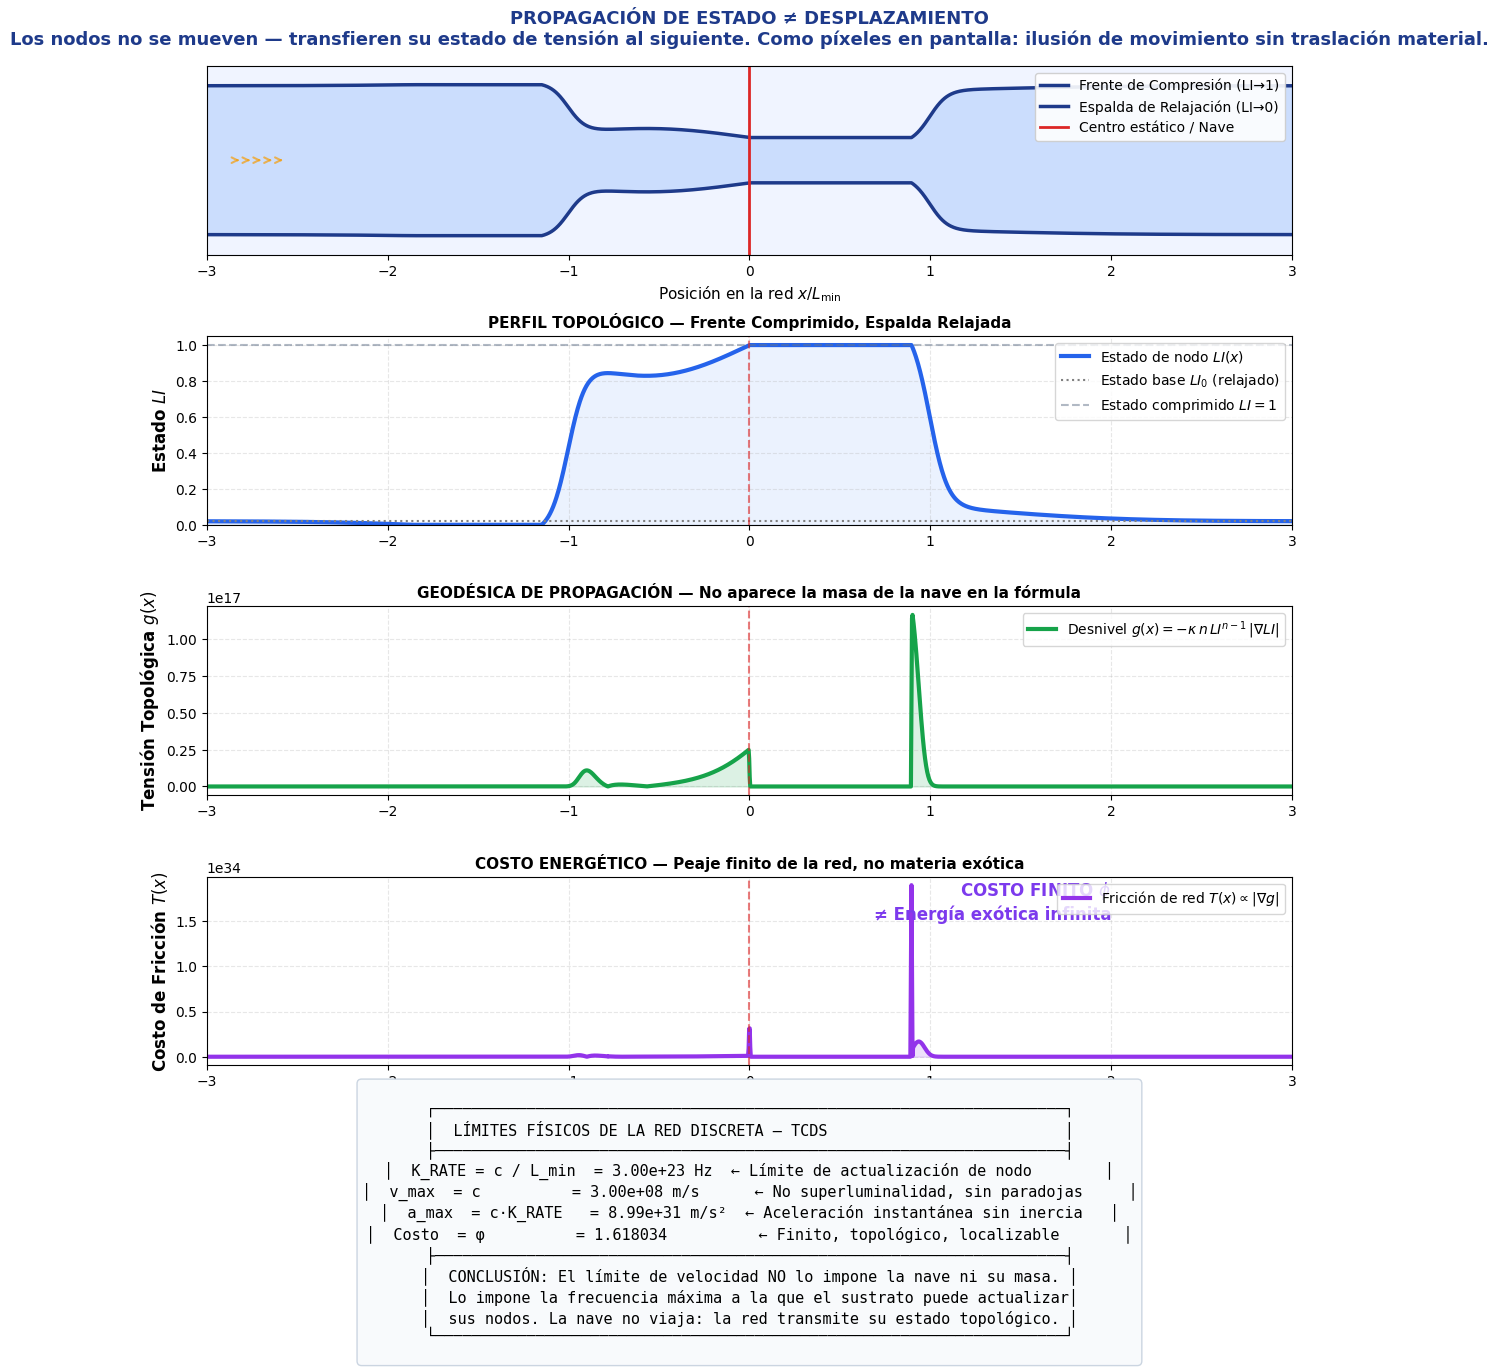
\includegraphics[width=0.92\linewidth]{descarga (52).png}
    \caption{Dinámica de propagación de estado frente a desplazamiento. El gradiente topológico transfiere tensión nodal sin traslación material.}
    \label{fig:propagacion}
\end{figure}

\section{Postulado V: Estabilidad Computacional del Marco Algebraico}
La viabilidad predictiva de esta red se ha validado mediante un pipeline algebraico vectorizado, el cual demuestra que los límites estructurales son invariantes ante la optimización computacional:
\begin{itemize}
    \item Actualización tradicional (bucle): $21\,786.00\,\mathrm{ms}$
    \item Actualización vectorizada (bloques): $0.23\,\mathrm{ms}$ (\textbf{Factor de aceleración: $96\,236.4 \times$})
\end{itemize}
La exactitud matemática entre ambos métodos es idéntica. La latencia del software no altera la física subyacente; únicamente demuestra la capacidad de simular densidades extremas respetando el límite $K_{\text{RATE}}$.

\begin{figure}[tbp]
    \centering
    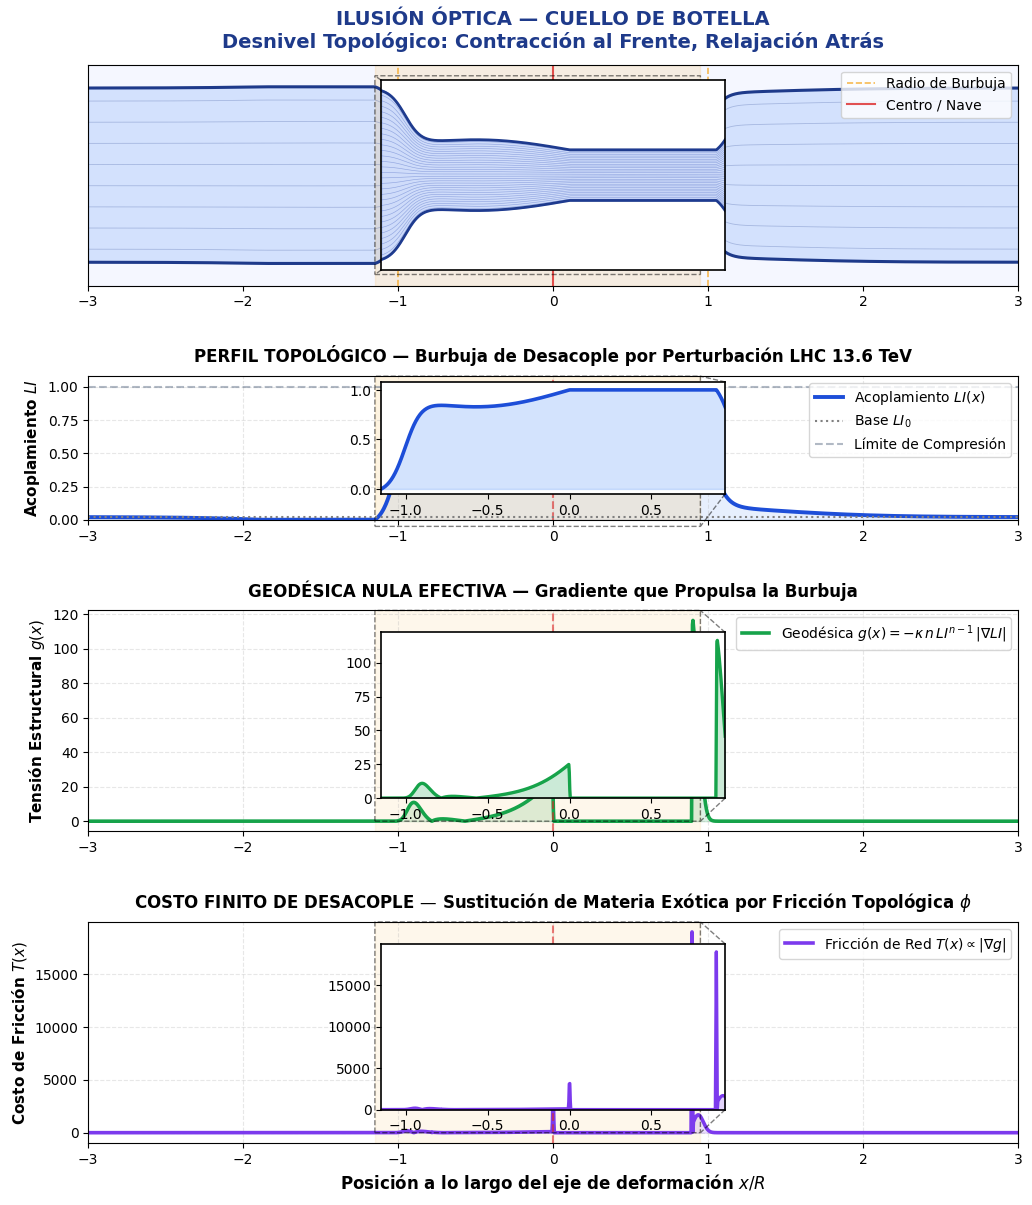
\includegraphics[width=0.92\linewidth]{descarga (51).png}
    \caption{Desnivel topológico y geodésica nula efectiva generada por el acoplamiento asimétrico del sustrato.}
    \label{fig:desnivel}
\end{figure}

\section{Física Convencional}
La divergencia principal respecto a la física relativista clásica se resume en el tratamiento de la inercia y el costo energético:

\subsection*{Física Clásica / Relatividad Especial (Desplazamiento Cinético)}
\begin{itemize}
    \item La masa se desplaza a través del espacio, requiriendo energía proporcional a $1/\sqrt{1 - v^2/c^2}$.
    \item La energía requerida diverge a infinito conforme $v \to c$.
    \item La aceleración genera fuerzas G letales, requiriendo tiempos de tránsito extendidos.
\end{itemize}

\subsection*{TCDS (Propagación en Red Discreta)}
\begin{itemize}
    \item El estado topológico se propaga (como un pulso en la red); no hay traslación local de masa.
    \item El costo energético es la fricción topológica $\varphi \approx 1.618$, manteniéndose finito a cualquier velocidad.
    \item Límite absoluto dictado por causalidad computacional ($K_{\text{RATE}}$), permitiendo una aceleración instantánea ($\Delta t \approx 3.34 \times 10^{-24}\,\mathrm{s}$).
\end{itemize}

\parrafoecuacion{par:intervalo-causal}{Intervalo de actualización}
El intervalo temporal citado en la comparación anterior es:
\begin{equation}
    \Delta t \approx 3.34 \times 10^{-24}\,\mathrm{s}.
    \label{eq:intervalo-causal}
\end{equation}

\section{Conclusión Final}
Bajo el marco de la TCDS, el modelo Warp deja de ser una estructura  irresoluble de densidades de energía negativas infinitas para convertirse en una posibilidad de \textbf{ingeniería topológica}: la viabilidad radica en la capacidad tecnológica de sincronizar la red lo suficientemente rápido para mantener el perfil asimétrico $LI(x)$ frente y detrás de la nave.
\subsection{Coherencia de parsimonia}
La viabilidad que se deriva de este marco no se limita al caso específico de la burbuja de deformación, sino que encuentra correspondencia con dos fenómenos que hasta ahora se trataban como dominios separados: la expansión cósmica y la estructura de horizontes de sucesos.

En la métrica de Alcubierre, la curvatura se construye como una asimetría local: contracción delante de la nave y expansión detrás de ella. Esta misma asimetría aparece en la dinámica de Hubble, donde el sustrato se expande de forma global y uniforme a gran escala. Bajo la interpretación de acoplamiento topológico, ambos fenómenos son manifestaciones del mismo mecanismo fundamental: un desequilibrio en el estado de tensión de la red discreta. En el caso Hubble, el acoplamiento global del sustrato disminuye de forma gradual en todas direcciones; en el caso warp, el desacople es localizado y asimétrico, concentrado en una región finita. Algebraicamente, ambos comparten la misma estructura: un gradiente de estado de acoplamiento que se propaga de nodo a nodo sin traslación material.

Esta identidad se extiende también a los horizontes de sucesos. En cualquier límite causal —sea el horizonte de un agujero negro, el horizonte cosmológico o el borde de la burbuja warp— lo que se observa no es una barrera física impenetrable, sino el límite de sincronización de la red: más allá de esa frontera, la actualización de estado no puede transmitirse al ritmo que requiere el perfil, y por tanto, la información se desacopla. En todos los casos, la ecuación fundamental \(Q \cdot \Sigma \cdot \tau_C = \phi\) se mantiene invariante. Lo que cambia es únicamente la distribución espacial del perfil de acoplamiento \(LI(x)\): uniforme y global en Hubble, localizada y asimétrica en la métrica de Alcubierre, y con frontera de desacople en horizontes de sucesos.

Se concluye que la viabilidad del mecanismo warp no es un caso aislado ni una invención ad hoc: es la manifestación localizada de la misma dinámica de acoplamiento que opera a escala cósmica y en fronteras causales. La métrica de Alcubierre no requiere física distinta a la que ya está presente en el universo observable; simplemente la organiza de forma asimétrica. El mismo tipo de acople del sustrato, gobernado por la ley de balance coherencial, opera en todos los dominios sin excepción, unificando la descripción de la expansión del universo, la estructura de horizontes y la propulsión por deformación del espacio-tiempo bajo un único principio algebraico.


\section{Glosario de ecuaciones}
\label{sec:glosario-ecuaciones}
Cada entrada enlaza con la ecuación numerada y con el párrafo identificado como P1, P2, etc., donde se explica su uso. Las páginas se actualizan automáticamente al compilar. Las descripciones resumen las relaciones presentadas en este documento.
\begin{description}[style=nextline,leftmargin=1em,labelindent=0pt,itemsep=5pt,parsep=0pt]
    \entradaecuacion{eq:lbcu}{par:lbcu}{Balance coherencial}
        {Relaciona $Q$, $\Sigma$, $\tau_C$ y $\phi$ en la LBCU.}
    \entradaecuacion{eq:phi}{par:phi}{Fricción topológica}
        {Especifica el valor de $\phi$ empleado en el marco algebraico.}
    \entradaecuacion{eq:tiempo-causal}{par:tiempo-causal}{Tiempo causal}
        {Expresa $\tau_C$ en función de $Q$, $\Sigma$ y $\phi$.}
    \entradaecuacion{eq:amplitud}{par:amplitud}{Amplitud base adimensional}
        {Relaciona la amplitud base adimensional $\kappa_{\text{base}}$ con $Q$ y $\phi$, antes de su proyección en unidades físicas.}
    \entradaecuacion{eq:exponente}{par:exponente}{Exponente de la red}
        {Especifica el exponente $n$ del perfil.}
    \entradaecuacion{eq:perfil}{par:perfil}{Perfil de acoplamiento}
        {Define $LI(x)$ a partir del estado base $LI_0$ y de $f(x)$.}
    \entradaecuacion{eq:forma}{par:forma}{Función de forma}
        {Expresa $f(x)$ mediante funciones tangente hiperbólica.}
    \entradaecuacion{eq:geodesica}{par:geodesica}{Geodésica de tensión}
        {Relaciona $g(x)$ con la amplitud base $\kappa_{\text{base}}$, el exponente $n$, el perfil $LI(x)$ y su derivada espacial.}
    \entradaecuacion{eq:costo}{par:costo}{Costo local}
        {Expresa $T(x)$ mediante la magnitud de la derivada de $g(x)$.}
    \entradaecuacion{eq:limite-causal}{par:limite-causal}{Límite causal}
        {Reúne la frecuencia de sincronización y la velocidad máxima propuestas.}
    \entradaecuacion{eq:longitud-minima}{par:longitud-minima}{Longitud mínima}
        {Fija el valor de $L_{\text{min}}$ adoptado en el documento.}
    \entradaecuacion{eq:velocidad-maxima}{par:velocidad-maxima}{Velocidad máxima}
        {Indica el valor numérico de $c$ empleado.}
    \entradaecuacion{eq:frecuencia-maxima}{par:frecuencia-maxima}{Frecuencia máxima}
        {Presenta el valor numérico de $K_{\text{RATE}}$.}
    \entradaecuacion{eq:velocidad-terminal}{par:velocidad-terminal}{Velocidad terminal}
        {Especifica la velocidad terminal propuesta para la burbuja.}
    \entradaecuacion{eq:aceleracion-maxima}{par:aceleracion-maxima}{Aceleración máxima}
        {Relaciona $a_{\text{max}}$ con $c$ y $K_{\text{RATE}}$.}
    \entradaecuacion{eq:intervalo-causal}{par:intervalo-causal}{Intervalo causal}
        {Recoge el intervalo $\Delta t$ citado en la comparación.}
\end{description}

\begin{thebibliography}{9}
    \small\raggedright
    \bibitem{alcubierre1994}
    M.~Alcubierre,
    ``The warp drive: hyper-fast travel within general relativity'',
    \textit{Classical and Quantum Gravity}, \textbf{11}(5), L73--L77 (1994).
    DOI: \href{https://doi.org/10.1088/0264-9381/11/5/001}{10.1088/0264-9381/11/5/001}.
    Texto disponible en \href{https://arxiv.org/abs/gr-qc/0009013}{arXiv:gr-qc/0009013}.
    \bibitem{alcubierre2008}
    M.~Alcubierre,
    \textit{Introduction to 3+1 Numerical Relativity}.
    Oxford University Press (2008).
    ISBN: 978-0-19-920567-7.
    \bibitem{zenodo22639220}
    Carrasco Ozuna, G. (2026).
    \textit{Teoría Cromodinámica Sincrónica --- TCDS: Pipeline de relación H--LI}
    (Version v1.0). Zenodo.
    DOI: \href{https://doi.org/10.5281/zenodo.22639220}{10.5281/zenodo.22639220}.
\end{thebibliography}

\end{document}
